\documentclass{article}

\usepackage{fullpage,latexsym,picinpar,amsmath,amsfonts,graphicx}

\input{macros.tex}

\begin{document}
\centerline{REMOVED}
\centerline{REMOVED}
\centerline{\large \bf CS/MATH111 ASSIGNMENT 4}
%\centerline{due Saturday, May 25 (11:50PM)}

\vskip 0.2in
%\noindent{\bf Individual assignment:} Problems 1 and 2.

%\noindent{\bf Group assignment:} Problems 1 and 2.

\vskip 0.1in

%%%%%%%%%%%%%%%%%%%%%%%%%%%%

\begin{problem}
a)
Give the asymptotic value (using the $\Theta$-notation)
for the number of letters that will be printed by the algorithms below.
In each algorithm the argument $n$ is a positive integer.
Your solution needs to consist of an appropriate recurrence 
equation and its solution. You also need to give a brief justification for
the recurrence (at most 10 words each). 

\bigskip
\noindent
(i)\ \ 
\begin{minipage}[t]{3in}
\begin{tabbing}
aaa \= aaa \= aaa \= aaa \=  \kill
\textbf{Algorithm} \textsc{PrintAs} $(n: \mbox{\bf integer})$ \\
          \> \textbf{if} $n < 4$ \\
          \>\>  print(``A") \\
          \>\textbf{else} \\
          \>\>  \textsc{PrintAs}$(\ceiling{n/3})$\\
          \>\>  \textsc{PrintAs}$(\ceiling{n/3})$\\
          \>\>  \textsc{PrintAs}$(\ceiling{n/3})$\\
          \>\>  \textsc{PrintAs}$(\ceiling{n/3})$\\
           \>\>  \textsc{PrintAs}$(\ceiling{n/3})$\\
      \>\> \textbf{for} $i \leftarrow 1$ \textbf{to} $4$ \textbf{do} print(``A")
\end{tabbing}
\end{minipage}

\bigskip
\noindent
(ii)\ \
\begin{minipage}[t]{3in}
\begin{tabbing}
aaa \= aaa \= aaa \= aaa \=  \kill
\textbf{Algorithm} \textsc{PrintBs} $(n: \mbox{\bf integer})$ \\
          \> \textbf{if} $n < 2$ \\
          \>\>  print(``B") \\
          \>\textbf{else} \\
          \>\>  \textbf{for} $j \leftarrow 1$ \textbf{to} $6$ 
					\textbf{do} \textsc{PrintBs}$(\floor{n/2})$\\
      \>\> \textbf{for} $i \leftarrow 1$ \textbf{to} $10n^3$ \textbf{do} print(``B")
\end{tabbing}
\end{minipage}

\bigskip
\noindent
(iii)\ \ 
\begin{minipage}[t]{3in}
\begin{tabbing}
aaa \= aaa \= aaa \= aaa \=  \kill
\textbf{Algorithm} \textsc{PrintCs} $(n: \mbox{\bf integer})$ \\
          \> \textbf{if} $n < 3$ \\
          \>\>  print(``C") \\
          \>\textbf{else} \\
          \>\>  \textsc{PrintCs}$(\ceiling{n/2})$\\
          \>\>  \textsc{PrintCs}$(\ceiling{n/2})$\\
          \>\>  \textsc{PrintCs}$(\ceiling{n/2})$\\
          \>\>  \textsc{PrintCs}$(\ceiling{n/2})$\\
      \>\> \textbf{for} $i \leftarrow 1$ \textbf{to} $20n^2$ \textbf{do} print(``C")
\end{tabbing}
\end{minipage}

\bigskip
\noindent
b) For each integer $n \ge 1$ we define a tree $T_n$, recursively, as follows. For $n=1$, $T_1$ is
a single node. For $n > 1$, $T_n$ is obtained from four copies of $T_{\ceiling{n/2}}$ and three
additional nodes, by connecting them as follows:
%
\begin{center}
%\includegraphics[width=3.5in]{HW_s19/treeforhw4.pdf}
\includegraphics[width=3.5in]{treeforhw4.pdf}
\end{center}
%
(In this figure, the subtrees are denoted $T_{n/2}$, without rounding, to reduce clutter.)
Let $h(n)$ be the number of nodes in $T_n$. Give a recurrence equation for $h(n)$ and
justify it. Then give the solution of this recurrence  using the $\Theta()$ notation.
\end{problem}

%%%%%%%%%%%%%%%%%%%%%%%%%%%%
\bigskip
\bigskip
\begin{solution}

\noindent
a).

(i)\ \ 
$T(n) = 5T(n/3) + 4$  with $\theta(n^{log_35})$:
There are 5 recursive calls with n/3 and a loop called 4 times.

\smallskip
(ii)\ \ 
$T(n) = 6T(n/2) + 10n^{3}$ with $\theta(n^{3})$:
6 Recursive calls with n/2 in first for loop and the next loop at
$10n^{3}$ 

\smallskip
(iii)\ \ 
$T(n) = 4T(n/2) + 20n^{2}$ with $\theta(n^{2}log(n))$:
There's 4 recursive calls with n/2 with a loop going to $n^{2}$

\smallskip
\noindent
b).

$h(n) = 4h(n/2) + 3$ with $\theta(n^{2})$:
There are 4 recursive calls with n/2 with 3 beginning nodes.
\end{solution}
%%%%%%%%%%%%%%%%%%%%%%%%%%%%
\begin{problem}
a) Bill is buying his wife a bouquet of daises, carnations, roses and tulips. 
The bouquet will have $25$ flowers, with 
%
\begin{itemize} 
		\item between $1$ and $7$ daises,
        \item between $2$ and $11$ carnations,
		\item at least $4$ roses, and
		\item at most $6$ tulips. 
\end{itemize}
%
How many different combinations of flowers satisfy these requirements?
You need to use the counting method for integer partitions and show your work.
%  \end{problem}



%%%%%%%%%%%%%%%%%%%%%%%%%%%%
\bigskip
%  \begin{problem}
\noindent 
b) We have three sets $P$, $Q$, $R$
with the following properties:

\begin{description}

\item{(a)}  $|Q| = 2|P|$ and 
                $|R| = 4|P|$,

\item{(b)} $|P\cap Q| = 11$,
        $|P\cap R| = 7$,
        $|Q\cap R| = 10$,

\item{(c)}
$1\le |P\cap Q\cap R| \le 11$,

\item{(d)}
$|P\cup Q\cup R| = 121$.

\end{description}

Use the inclusion-exclusion principle to
determine the number of elements in $P$.
Show your work.
(Hint: You may get an equation with two unknowns, but one of them has only a few possible values.)
\end{problem}



%%%%%%%%%%%%%%%%%%%%%%%%%%%%

\begin{solution}
\newline
a.)
\newline
Key:
\newline
c = carnations
\newline
d = daises
\newline
r = roses
\newline
t = tulips
\newline
\newline
In order to achieve 25 flowers, we must add all the flowers together.
\newline
$c+d+r+t=25$
\newline
Daises: $1 \leq d \leq 7$
\newline
Carnations: $2 \leq c \leq 11$
\newline
Roses: $r \geq 4$
\newline
Tulips: $t \leq 6$
\newline
\newline
We then remove lower bounds, which would achieve the following:
\newline
Daises: $d' = d - 1$
\newline
$d \leq 6$
\newline
Carnations: $c' = c - 2$
\newline
$c \leq 9$
\newline
Roses: $r \geq 3$
\newline
Tulips: $t \leq 6$
\newline
\newline
Now, we plug in the variables using the formulas provided from the "Or's of lower bounds" slides in Inclusion-Exclusion:
\newline
\newline
$S(c'\leq 9 \cap d \leq 6 \cap t' \leq 6) = S - S(c' \geq 10 \cup d \geq 7 \cup t' \geq 7)$
\newline
\newline
${m+k-1\choose k-1}$ = ${21\choose3}$ = $1330$
\newline
\newline
$S(c' \geq 10 \  \cup \ d \geq 7 \  \cup \ t' \geq 7) = S(c' \geq 10) + S(d \geq 7) + S(t' \geq 7)
\newline
- S(c' \geq 10 \  \cap \ d \geq 7) - S(c' \geq 10 \  \cap \ t' \geq 7) - S(d \geq 7 \  \cap \ t' \geq 7) + S(c' \geq 10 \  \cap \ d \geq 7 \  \cap \ t' \geq 7) 
\newline
\newline
= {18 - 10 + 3 \choose 3} + {18 - 7 + 3 \choose 3}  + {18 - 7 + 3 \choose 3}  - {18 - 10 - 7 + 3 \choose 3} - {18 - 10 - 7 + 3 \choose 3}  - {18 - 7 - 7 + 3 \choose 3} + {18 - 10 - 7 - 7 + 3 \choose 3}
\newline
= {11 \choose 3} + {14 \choose 3} + {14 \choose 3} - {4 \choose 3} - {4 \choose 3} - {7 \choose 3} + {-3 \choose 3} \\$
\newline
So $165 +364 + 364 -4 -4 -35 = 850$
\newline
Then $1330-850 = 480$ total combinations
\newline
\newline
\newline
b.) Using the inclusion-exclusion principle to determine the number of elements in P, we get the following below from the slides:
\newline
\left\vert{P\cup Q\cup R}\right\vert & = \left\vert{P}\right\vert + \left\vert{Q}\right\vert + \left\vert{R}\right\vert - \left\vert{P \cap Q}\right\vert - \left\vert{P \cap R}\right\vert - \left\vert{Q \cap R}\right\vert + \left\vert{P \cap Q \cap R}\right\vert \\

\newline
\newline
We now plug in the variables given from the problem into the equation:

121 = \left\vert{P}\right\vert + 2\left\vert{P}\right\vert + 4\left\vert{P}\right\vert - 11 - 7 - 10 + \left\vert{P \cap Q \cap R}\right\vert$ \\
\newline
We now simplify from here:
\newline
121 & = 7\left\vert{P}\right\vert - 28 + \left\vert{P \cap Q \cap R}\right\vert \\
149 & = 7\left\vert{P}\right\vert + \left\vert{P \cap Q \cap R}\right\vert \\$
\newline
We now move 7\left\vert{P}\right\vert$ to the opposite side in order to solve for \left\vert{P}\right\vert$ below:
\newline
7\left\vert{P}\right\vert & = 149 - \left\vert{P \cap Q \cap R}\right\vert \\
\left\vert{P}\right\vert & = \dfrac{149 - \left\vert{P \cap Q \cap R}\right\vert}{7} \\
\newline
$We need to now solve for the integer of $\left\vert{P}\right\vert$. With the information we have, we can take a look at the equation $1\le |P\cap Q\cap R| \le 11$ and determine two possible outcomes below:
\newline
\newline
$\left\vert{P \cap Q \cap R}\right\vert = 2$ or $9$.
\newline
\newline
When looking at $\left\vert{P \cap R}\right\vert = 7$, we realize $\left\vert{P \cap Q \cap R}\right\vert$ goes past 7, and thus $\left\vert{P \cap Q \cap R}\right\vert = 9$.
\newline
We then plug in the values into the final equation:
\newline
\newline
$\left\vert{P}\right\vert = \dfrac{149 - 2}{7} = \dfrac{147}{7} = 21
\end{solution}

\vskip 0.1in
\paragraph{Submission.}
To submit the homework, you need to upload the pdf file into Gradescope and iLearn .


\end{document}

